%% aps to author template--please use pdflatex to edit then to pdf--------------
\documentclass[A4,twoside,fontset=ubuntu,UTF8]{ctexart}
%\usepackage{slashbox}\usepackage{makecell}\usepackage{diagbox}\backslashbox
\usepackage{aappss}
%\usepackage{epstopdf}

\newcommand{\vx}{{\mathbf{x}}}
%\renewcommand\baselinestretch{1.235}\protect
\renewcommand\baselinestretch{2.0}\protect
\abovedisplayshortskip 0 pt plus 3pt
\belowdisplayshortskip 6 pt plus 2pt minus 2pt
\abovedisplayskip 6 pt plus 2pt minus 2pt
\belowdisplayskip 6 pt plus 2pt minus 2pt
% \info{2015}{64}{1}{01{}} \infodate{2015.0.0.}{2015.0.0.}
%=================== Text begin here ==============================
\begin{document}\apsname

\title{自动微分与编程语言 \fivestar}%{\cfundlink}

\author{刘金国$^{1)}$ \quad 许开来$^{2)}$}

\address{1)}{哈佛大学物理系, 波士顿 \quad 02138}
\address{2)}{...}

%\address{3)}{}

\abstract{自动微分是机器学习中核心的数值技术。机器学习中用到的自动微分主要是以张量层面的微分居多,其衍生的工具可以解决张量网络等算法的变分优化。而本文主要介绍另外一种更加通用的,在编程语言层面的自动微分,并介绍它在科学计算中的用途和未来发展的趋势。}

\keywords{自动微分,科学计算,编程语言}

% https://ufn.ru/en/pacs/all/
% 02.60.Pn numerical optimization
% 02.30.Jr Partial differential equations
\pacs{02.60.Pn, 02.30.Jr}

\cfund{}

\cmail{cacate0129@gmail.com \quad }

%\cmailddag{mail2}

%\mail{}{}\cmail \cmailddag

%\apscopyright \baselineskip=16.0pt plus.2pt minus.2pt
%\begin{multicols}{2}\sec
\vskip 0.55\baselineskip
\section{引~~~~言}
自动微分是指自动获取一个目标计算机程序导数的技术。
与很多人印象不同的是,自动微分是个十分有年代的技术。
Nolan曾在他1953年的博士论文中就提出过~\cite{Nolan1953}自动化求导计算机程序的构想,
它利用了计算机程序的一个普遍特性,那就是不管程序有多么复杂,总可以被分解成加减乘除之类的基础指令。
我们很容易知晓基础指令的自动微分规则,因而可以通过简单的链式法则推导出整个程序的导数。
    在上世纪60年代,自动微分发展出了两种不同的实践,一种叫做前向传播(Forward propagation)~\cite{Wengert1964},一种叫做后向传播(Backward propagation)~\cite{Boltyanski1960}。
一个计算过程 $f : \mathbb{R}^m \rightarrow \mathbb{R}^n$可以被描述为
\begin{align*}
    &\vx^1 = f_1(\vx^0)\\
    &\vx^2 = f_2(\vx^1)\\
    &\ldots\\
    &\vx^L = f_L(\vx^{L-1})
\end{align*}
其中 $x^0\in R^m$, $x^L\in R^n$, $L$是计算的步骤数。
这段程序的雅可比 (Jacobian) 矩阵$J_{ij} \equiv \frac{\partial x^L_i}{\partial x_j^0}$是一个$n\times m$的矩阵,其中$x_j^0$和$x_i^L$代表了输入和输出中的一个元素。
前向自动微分的链式法则表述为$\frac{\partial \vx^k}{\partial x^0_j} = \frac{\partial \vx^k}{\partial \vx^{k-1}}\frac{\partial \vx^{k-1}}{\partial x^0_j}$,它计算了雅可比矩阵的第$j$列。后向自动微分的链式法则为$\frac{\partial \vx^L_i}{\partial x^{k-1}} = \frac{\partial \vx^L_i}{\partial \vx^{k}}\frac{\partial \vx^{k}}{\partial x^{k-1}}$,它计算了雅可比矩阵的第$i$行。不难发现,它们梯度的传递计算方向分别是向前和向后,这也决定了它们的实现难度。

过去,很多机器学习中的神经元网络往往由简单的几种定义在张量上的操作构成,因此人们很容易手推出一个常用函数族的导数。但最近几年,机器学习界风靡起了微分编程。因为大家认识到神经元网络的固定的函数族(矩阵乘法,卷积函数,relu函数等)已经开始渐渐满足不了神经元网络多样性的设计,我们需要把自动微分当作“一等公民”的编程语言。
类似的需求在物理中也很多见,比如在张量网络等模拟中需要用到的复数奇异值分解函数\cite{Wan2019,Liao2019},严格对教化求解基态过程中用到的极大极小本正值求解器~\cite{Xie2020},模拟变分量子算法中幺正量子线路的求导~\cite{Luo2019}。
人们为了手推这些求导规则付出了很多的努力,如果我们有了编程语言层面的自动微分,那么这些都可以在程序编写之时就得到解决。

\vskip 1.55\baselineskip
\section{自动微分在科学计算领域的应用}

\vskip 1.55\baselineskip
\subsection{地震波的模拟}

\vskip 1.55\baselineskip
\subsection{热带(Tropical)张量网络求解自旋玻璃最优构型}
热带张量网络是张量网络的一个特别的应用,它重新定义了张量中基础元素的代数为
\begin{eqnarray}
x \oplus y  = \max(x, y),\,\,\,\,\,\,\,\,\,\,\,\, \,\,\,\,
x \odot y   =  x + y. \label{eq:max-sum-alg}
\end{eqnarray}
\begin{figure}[t]
\centering
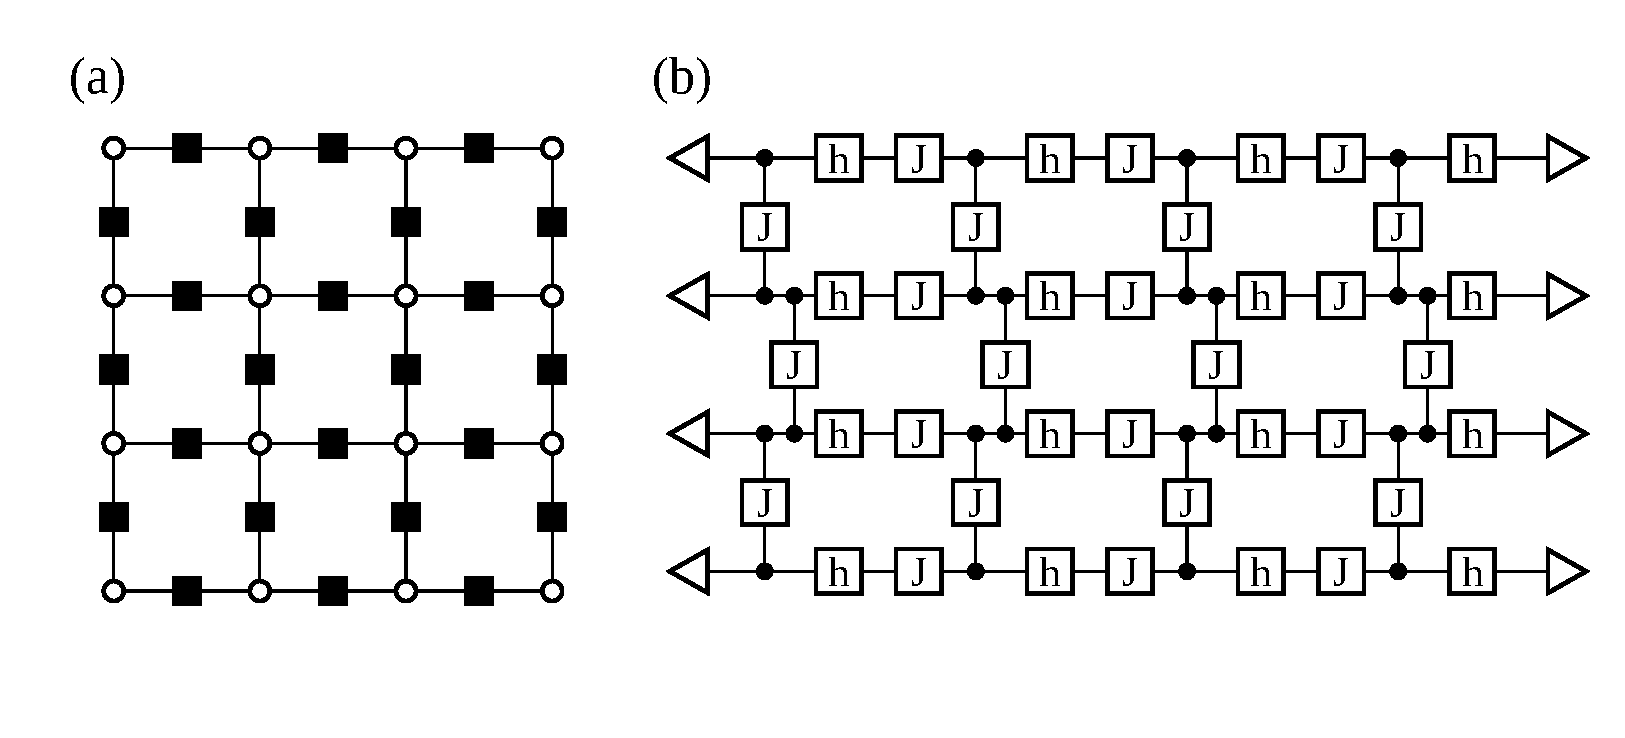
\includegraphics[width=\columnwidth]{./transform12.pdf}
    \caption{正方晶格上的自旋玻璃问题,(a)对应的热带张量网络表示。(b)对应的“量子线路”表示。\label{fig:performance}} 
\end{figure}
如果我们将张量中的元素定义为自旋玻璃的耦合强度,我们就可以通过收缩这个张量结构得到自旋玻璃的最优构型。
这个最优构型的能量表达式为
\begin{equation}
    E(\{\sigma\}) = \max\limits_{\sigma}-\sum_{i < j }J_{ij} \sigma_i \sigma_j  - \sum_i h_i \sigma_i,
\label{eq:spinglassopt}
\end{equation}
    因此对它的微分就是。
但是作了这样的替换,张量收缩的微分规则就发生了变换。

\vskip 0.55\baselineskip
\section{自动微分与可逆计算}

自动微分

\section{结~~~~论}

\section*{致谢}

感谢北京大学力学系某某教授和某某博士以及某某的讨论.


\section*{附录A1}

标题排列和编号方式为A1, A2, A3.

\section*{附录A2}
%
%text text
%
%\section*{附录B1}
%%\section*{附录B2}
%
%text text
%
%\section*{致谢}
%
%text text

\bigskip
%\begin{footnotesize}

\bibliographystyle{apsrev4-1}
\bibliography{invc}

\newpage

\title{English Title $^{\ast}$}%{\efundlink}

\efund{Project supported by the State Key Development Program for Basic Research of China (Grant No. 2011CB00000), the National Natural Science Foundation of China (Grant Nos. 123456, 567890), and the National High Technology Research and Development Program of China (Grant No. 2011AA06Z000). \\}


\author{Guan Yun-Chang$^{1)2)}$ \quad  Liu Bei$^{1)\dag}$ \quad  Zhuge Liang$^{2)}$}

\email{aaa@bbb.ccc  }
%\email \emailddag


\eaddress{1)}{State Key Laboratory of Quantum Optics and Quantum Optics  Devices,
Institute of Opto-Electronics, Shanxi University, Taiyuan 030006, China}

\eaddress{2)}{Department of Physics, Tsinghua University, Beijing 100084, China}

\eabstract{}

\small  To determine the probe made of amino acids arranged in a linear chain and joined together by peptide bonds between the carboxyl and amino groups of adjacent amino acid residues. The sequence of amino acids in a protein is defined by a gene and encoded in the genetic code. This can happen either
before the protein is used in the cell, or as part of control mechanisms.

\ekeywords{Keyword1, Keyword2, Keyword3, Keyword4 \\}

\epacs{02.10.Yn, 33.15.Vb, 98.52.Cf, 78.47.dc}

\end{document}
